\documentclass[paper=a4, fontsize=11pt]{scrartcl} 

\usepackage[T1]{fontenc} 
\usepackage[english]{babel}
\usepackage{amsmath,amsfonts,amsthm}

\usepackage{lipsum}

\usepackage{graphicx}
\usepackage{float}
  \floatplacement{figure}{H}
  \floatplacement{table}{H}
  
\usepackage{sectsty} 
\allsectionsfont{\centering \normalfont\scshape} 

\usepackage{fancyhdr} % Custom headers and footers
\pagestyle{fancyplain} % Makes all pages in the document conform to the custom headers and footers
\fancyhead{} % No page header - if you want one, create it in the same way as the footers below
\fancyfoot[L]{} % Empty left footer
\fancyfoot[C]{} % Empty center footer
\fancyfoot[R]{\thepage} % Page numbering for right footer
\renewcommand{\headrulewidth}{0pt} % Remove header underlines
\renewcommand{\footrulewidth}{0pt} % Remove footer underlines
\setlength{\headheight}{13.6pt} % Customize the height of the header

\usepackage[labelformat=empty]{caption}
\usepackage{color}
\usepackage{listings}
\lstset{ %
language=bash,                % choose the language of the code
basicstyle=\footnotesize,       % the size of the fonts that are used for the code
numbers=left,                   % where to put the line-numbers
numberstyle=\footnotesize,      % the size of the fonts that are used for the line-numbers
stepnumber=1,                   % the step between two line-numbers. If it is 1 each line will be numbered
numbersep=5pt,                  % how far the line-numbers are from the code
backgroundcolor=\color{white},  % choose the background color. You must add \usepackage{color}
showspaces=false,               % show spaces adding particular underscores
showstringspaces=false,         % underline spaces within strings
showtabs=false,                 % show tabs within strings adding particular underscores
frame=single,           % adds a frame around the code
tabsize=2,          % sets default tabsize to 2 spaces
captionpos=b,           % sets the caption-position to bottom
breaklines=true,        % sets automatic line breaking
breakatwhitespace=false,    % sets if automatic breaks should only happen at whitespace
escapeinside={\%*}{*)}          % if you want to add a comment within your code
}
\usepackage{hyperref}


\numberwithin{equation}{section} % Number equations within sections (i.e. 1.1, 1.2, 2.1, 2.2 instead of 1, 2, 3, 4)
\numberwithin{figure}{section} % Number figures within sections (i.e. 1.1, 1.2, 2.1, 2.2 instead of 1, 2, 3, 4)
\numberwithin{table}{section} % Number tables within sections (i.e. 1.1, 1.2, 2.1, 2.2 instead of 1, 2, 3, 4)

\setlength\parindent{0pt} % Removes all indentation from paragraphs - comment this line for an assignment with lots of text

%----------------------------------------------------------------------------------------
%	TITLE SECTION
%----------------------------------------------------------------------------------------

\newcommand{\horrule}[1]{\rule{\linewidth}{#1}} % Create horizontal rule command with 1 argument of height

\title{	
\normalfont \normalsize 
\textsc{Computational Science} \\ [25pt] % Your university, school and/or department name(s)
\horrule{0.5pt} \\[0.2cm] % Thin top horizontal rule
\small Homework - Introduction to Frontiers of Computational Science\\ % The assignment title
%\horrule{2pt} \\[0.5cm] % Thick bottom horizontal rule
}

\author{\small{Ridlo W. Wibowo || 1215011069}} % Your name

\date{\small\today} % Today's date or a custom date


\begin{document}
\maketitle % Print the title

\textbf{Problem 1.}\\
Solve this simple oscillator equation.
\begin{equation*}
m \ddot{x} = -k x
\end{equation*}
with initial condition $x(0) = 1$ and $\dot{x}(0) = 0$, theoretically and numerically.\\

\textbf{Theoretically}\\
general solution for a function $x = e^{rt}$
\begin{eqnarray*}
\frac{d^{2}x}{dt^2} + \frac{k}{m}x &=& 0 \\
r^2e^{rt} + \frac{k}{m}e^{rt} &=& 0 \\
e^{rt} ( r^2 + \frac{k}{m}) &=& 0 \\
r^2 + \frac{k}{m} &=& 0 \\
r &=& \pm \sqrt{-\frac{k}{m}} = \pm i \sqrt{\frac{k}{m}} \\
r &=& \pm i \omega
\end{eqnarray*}
so the general solution by linear combination is
\begin{equation*}
x(t) = c_1 e^{+i \omega t} + c_2 e^{- \omega t}
\end{equation*}
rewrite above equation using euler formula
\begin{eqnarray*}
x(t) &=& (c_1 + c_2) \cos(\omega t) + i(c_1 - c_2)\sin(\omega t)\\
x(t) &=& A\cos(\omega t) + B\sin(\omega t)
\end{eqnarray*}
or we can use simpler form:
\begin{eqnarray*}
x(t) &=& C\cos(\omega t + \varphi)\\
\dot{x}(t) &=& -C \omega \sin(\omega t + \varphi)
\end{eqnarray*}
using the initial condition we will get the solution:
\begin{equation*}
x(t) = \cos(\omega t)
\end{equation*}

\textbf{Numerically}\\
we can use Taylor expansions:
\begin{eqnarray*}
x(t + \Delta t) &=& x(t) + v(t)\Delta t + \frac{a(t) \Delta t^2}{2} + \frac{b(t) \Delta t^3}{6} + \mathcal{O}(\Delta t^4)\\
x(t - \Delta t) &=& x(t) - v(t)\Delta t + \frac{a(t) \Delta t^2}{2} - \frac{b(t) \Delta t^3}{6} + \mathcal{O}(\Delta t^4)
\end{eqnarray*}
where $x$ is the position, $v = \dot{x}$ the velocity, $a = \ddot{x}$ the acceleration and $b$ the jerk (third derivative of the position with respect to the time) t.\\
Adding these two expansions gives
\begin{equation*}
x(t + \Delta t) = 2x(t) - x(t - \Delta t) + a(t)\Delta t^2 + \mathcal{O}(\Delta t^4).
\end{equation*}
this method which is so called Verlet algorithm is an order more accurate than integration by simple Taylor expansion alone because we can see that the first and third-order terms from the Taylor expansion cancel out.\\
for this problem $a(t) = -\omega^2 x(t)$, and using this method we need two position for one iteration, so for the first time step we can use Taylor expansion to get the position
\begin{equation*}
x_1 = x_0 + v_0 \Delta t + \frac{1}{2} a_0 \Delta t^2 (\mathcal{O}(\Delta t^3))
\end{equation*}
The error is not considered a problem because on a simulation of over a large amount of timesteps, the error on the first timestep is only a negligibly small amount of the total error.\\

Calculation using initial condition above with $\omega = 10$ and $\Delta t = 0.01$ (10 periods):
\begin{figure}
	\centering
	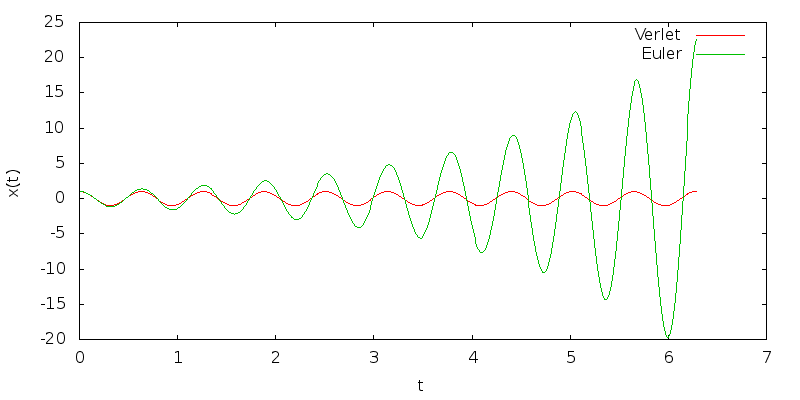
\includegraphics[width=0.7\textwidth]{verlet.png}
	\caption{Comparison between Verlet and Euler method for the same problem.}
\end{figure}

Calculation using Verlet algorithm with different $\Delta t$:
\begin{figure}
	\centering
	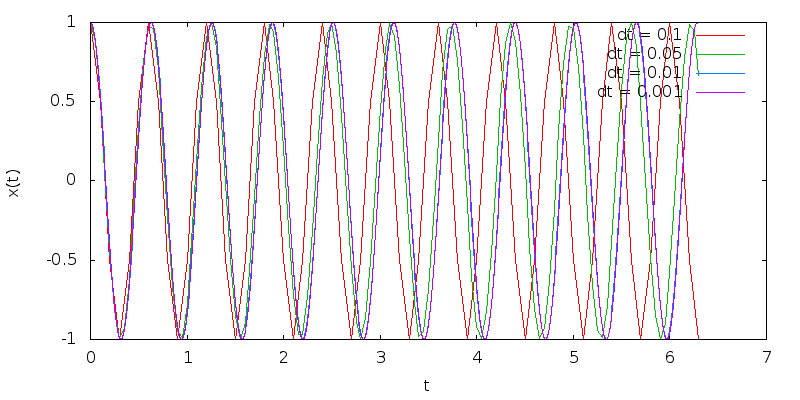
\includegraphics[width=0.8\textwidth]{verlet2.png}
	\caption{Comparison of the result from Verlet algorthm using different $\Delta t$.}
\end{figure}


\textit{\textbf{Program}}
\lstset{frameround=fttt}
\begin{lstlisting}
#include <iostream>
#include <stdlib.h>
#include <math.h>
#include <fstream>
using namespace std;

void plot();
int main(){
    double omega = 10.;
    double x0 = 1.;
    double v0 = 0.;
    double ti = 0., tf = 2.*M_PI;
    double dt = 0.01, x=x0, v=v0, t=ti, prev, next, a;

    double N = (tf - ti)/dt;
    
    // Verlet method
    ofstream out("output.txt");
    out << t << " " << x << endl;
    a = -1.*omega*omega*x; 
    prev = x;
    next = x + v*dt + 0.5*a*dt*dt; 
    t = t+dt;
    out << t << " " << next << endl;
    for (int i=1; i<=N; i++){
        a = -1*omega*omega*next;
        x = 2*next - prev + a*dt*dt;
        prev = next; 
        next = x; 
        t = t+dt;
        out << t << " " << x << endl;
    }
    out.close();
    
    // Euler method
    ofstream out2("output2.txt");
    x=x0; v=v0; t=ti;
    out2 << t << " " << x << endl;
    for (int i=0;i<=N;i++){
        a = -1.*omega*omega*x;
        x = x + v*dt;
        v = v + a*dt;
        t = t + dt;
        out2 << t << " " << x << endl;
    }
    out2.close();

    plot();
    return 0;
}

void plot(){
    ofstream ploter("inp.plt");
    ploter << "#gnuplot input file\n";
    ploter << "set term png size 600,400\n";
    ploter << "set output \"verlet.png\"\n";
    ploter << "set xlabel \"t\"\n";
    ploter << "set ylabel \"x(t)\"\n";
    ploter << "plot \"output.txt\" u 1:2 w l t \"Verlet\", \"output2.txt\" u 1:2 w l t \"Euler\"\n";
    ploter.close();

    system("gnuplot inp.plt");
}
\end{lstlisting}

\end{document}